\documentclass[a4paper,10pt]{article}
%\usepackage[T1]{fontenc}
\usepackage[utf8]{inputenc}
\usepackage[swedish]{babel}
\usepackage{color}
\usepackage{graphics}

\title{Webbteknik för ingenjörer \\
	Laboration 0}
\author{John-Patrik Nilsson \\
	e-mail: jpatrik.nilsson@gmail.com \\
	Skype: j-p.nilsson}

\begin{document}

\maketitle
%\tableofcontents

\pagestyle{empty}
\thispagestyle{empty}

\section{Inledning och problembeskrivning}
Laboration 0 var en introduktion till de kommunikationsverktyg Umeå Universitet använde vid sina distanskurser. Deltagare förväntades installera och lära sig hantera följande verktyg:
\begin{itemize}
\item Skype -- voice over IP/instant messaging.
\item Moodle -- Primärt kommunikationsverktyg mellan deltagarna på kursen, användes också som redovisningsverktyg.
\item VNC -- Virtual Network Computing, användes som redovisnings- och hjälpverktyg.
\end{itemize}

Platformen som användes för denna laboration är en persondator med operativsystemet Gentoo GNU/Linux med en 2.6.25 kärna. Således användes också Linuxversionerna av ovanstående kommunikationsverktyg.

\section{Moodle}
Moodle var det dynamiska webbsystem som användes som samlingsplats och kommunikationsverktyg av Umeå Universitet vid denna laboration. Detta webbsystem innehöll bl.a. forum, kalender, inlämningsverktyg, profiler och bloggar av och med deltagarna, samt litteratursförslag. 

För att som deltagare i kursen kunna använda Moodle behövde man först registrera sig som användare och deltagare i kursen, så en fungerande e-mail krävdes, samt ett registreringslösenord som var specifik för kursen. Detta lösenord visade sig stå på kursens statiska websida. 

Registreringsprocessen var snabb, och användingen av Moodle föreföll sig vara inituativ och rättfram. Det som var tvetydigt med hela systemet var att nödvändig information om kursen och dess innehåll var uppdelad på två olika webbsystem, dels Moodle, och dels kursens statiska hemsida, vilket gjorde det betydligt mindre smidigt att använda.

\section{Skype}
Skype var en applikation som tillhandahöll digital kommunikation över IP i såväl textform som ljudform. För användningen Skype behövdes ett upprättande av en Skype-konto vilket krävde att man angav sin e-mailaddress samt sitt prefererade smeknamn inom Skype-systemet. Registreringen och användningen av Skype var även den smidig och inituativ, och för att testa funktionaliteten av kommunikationsverktyget samt för att förbereda för efterföljande laborationer och övningar letades kursens handledares Skype-addresser upp och lades till i kontaktlistan.

\section{VNC}
VNC, eller Virtual Network Computing, är ett system vilket erbjuder avlägsen nätverksaccess till grafiska persondator-skrivbord. Till den persondator som användes vid denna laboration installerades VNC-programpaketet TightVNC. Installationen lick lätt och smidigt. Vid första uppstarten av serverprogrammet fick man ange det/de lösenord som skulle användas vid användning. Vid laborationen startades först serverprogrammet upp. För att sedan testa funktionaliteten startades även klientprogrammet upp och anslöts till serverprogrammet på samma arbetsstation. Förvisso testades inte nätverksaccessen från/till en avlägsen arbetsstation, men det är, tekniskt sett, ingen stor skillnad. Vid ett eventuellt scenario då avlägsen access är behövd krävs det att systemens brandväggar är konfigurerade på ett sådant sätt att kontakt kan etableras.

Programmen (server- och klientprogrammet) startades vid laborationen enligt följande kommandon från en terminal:
\\
\\
\fbox{\parbox{12cm}{
\textsl{(Med detta kommando beordrades serverapplikationen att beordra X-skrivbordsservern att starta ett nytt skrivbord som kunde nås via VNC klientapplikationer)} \\
\textcolor{blue}{\texttt{vncserver :1}}
\\
\\
\textsl{(Med detta kommando startades och anslöts VNC klientapplicationen till det nya skrivbordet via serverapplikationen)} \\
\textcolor{blue}{\texttt{vncviewer localhost:1}} }}
\\
\\
\\
Det avlägsna skrivbord som därefter visades via klientapplikationen såg deprimmerande tomt ut, endast en terminal sågs.

\appendix
\section{Screenshot}
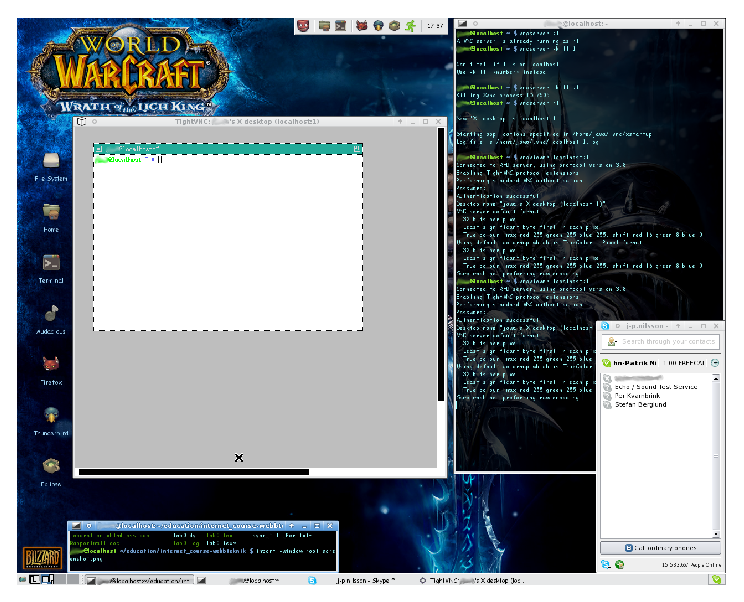
\includegraphics{screenshot.eps}

\section*{Referenser}
\textit{http://www.moodle.tfe.umu.se/} \\
\textit{http://www.tfe.umu.se/courses/systemteknik/webbkurser/wtfi/index.shtml} \\
\textit{http://www.tightvnc.com/} \\

\end{document}
